%%%%%%%%%%%%%%%%%%%%%%%%%%%%%%%%%%%%%%%%%
% Jacobs Landscape Poster
% LaTeX Template
% Version 1.0 (29/03/13)
%
% Created by:
% Computational Physics and Biophysics Group, Jacobs University
% https://teamwork.jacobs-university.de:8443/confluence/display/CoPandBiG/LaTeX+Poster
% 
% Further modified by:
% Nathaniel Johnston (nathaniel@njohnston.ca)
%
% This template has been downloaded from:
% http://www.LaTeXTemplates.com
%
% License:
% CC BY-NC-SA 3.0 (http://creativecommons.org/licenses/by-nc-sa/3.0/)
%
%%%%%%%%%%%%%%%%%%%%%%%%%%%%%%%%%%%%%%%%%

%----------------------------------------------------------------------------------------
%	PACKAGES AND OTHER DOCUMENT CONFIGURATIONS
%----------------------------------------------------------------------------------------

\documentclass[final]{beamer}

\usepackage[scale=1.24]{beamerposter} % Use the beamerposter package for laying out the poster

\usetheme{confposter} % Use the confposter theme supplied with this template

\setbeamercolor{block title}{fg=nred,bg=white} % Colors of the block titles
\setbeamercolor{block body}{fg=black,bg=white} % Colors of the body of blocks
\setbeamercolor{block alerted title}{fg=white,bg=dgreen!70} % Colors of the highlighted block titles
\setbeamercolor{block alerted body}{fg=black,bg=dgreen!10} % Colors of the body of highlighted blocks
% Many more colors are available for use in beamerthemeconfposter.sty

%-----------------------------------------------------------
% Define the column widths and overall poster size
% To set effective sepwid, onecolwid and twocolwid values, first choose how many columns you want and how much separation you want between columns
% In this template, the separation width chosen is 0.024 of the paper width and a 4-column layout
% onecolwid should therefore be (1-(# of columns+1)*sepwid)/# of columns e.g. (1-(4+1)*0.024)/4 = 0.22
% Set twocolwid to be (2*onecolwid)+sepwid = 0.464
% Set threecolwid to be (3*onecolwid)+2*sepwid = 0.708

\newlength{\sepwid}
\newlength{\onecolwid}
\newlength{\twocolwid}
\newlength{\threecolwid}
\setlength{\paperwidth}{48in} % A0 width: 46.8in
\setlength{\paperheight}{36in} % A0 height: 33.1in
\setlength{\sepwid}{0.024\paperwidth} % Separation width (white space) between columns
\setlength{\onecolwid}{0.22\paperwidth} % Width of one column
\setlength{\twocolwid}{0.464\paperwidth} % Width of two columns
\setlength{\threecolwid}{0.708\paperwidth} % Width of three columns
\setlength{\topmargin}{-0.5in} % Reduce the top margin size
%-----------------------------------------------------------

\usepackage{graphicx}  % Required for including images

\usepackage{booktabs} % Top and bottom rules for tables
\usepackage{multicol}
\usepackage{array}
\usepackage[font=small,skip=0pt]{caption}

%----------------------------------------------------------------------------------------
%	TITLE SECTION 
%----------------------------------------------------------------------------------------

\title{Malicious Browser Extensions} % Poster title

\author{Shishir Jindal, Tanmay Tiwari, Yogesh Biyani } % Author(s)

\institute{Department of Computer Science and Engineering, Indian Institute of Technology Roorkee} % Institution(s)


%----------------------------------------------------------------------------------------

\begin{document}
\addtobeamertemplate{headline}{} 
{
\begin{tikzpicture}[remember picture,overlay] 
\node [shift={(-10 cm,-5.8cm)}] at (current page.north east) {
\includegraphics[height=10cm]{logo.jpg}}; 
\end{tikzpicture} 
}
\addtobeamertemplate{block end}{}{\vspace*{2ex}} % White space under blocks
\addtobeamertemplate{block alerted end}{}{\vspace*{2ex}} % White space under highlighted (alert) blocks

\setlength{\belowcaptionskip}{2ex} % White space under figures
\setlength\belowdisplayshortskip{2ex} % White space under equations

\begin{frame}[t] % The whole poster is enclosed in one beamer frame

\begin{columns}[t] % The whole poster consists of three major columns, the second of which is split into two columns twice - the [t] option aligns each column's content to the top

\begin{column}{\sepwid}\end{column} % Empty spacer column

\begin{column}{\onecolwid} % The first column

%----------------------------------------------------------------------------------------
%	OBJECTIVES
%----------------------------------------------------------------------------------------

\begin{alertblock}{Abstract}
Through this paper, we project our work on the domain of Analysis of Malicious Browser Extensions for their classification and detection. There has been already a lot of work done on the detection of Native malware programs but no substantial research on Malicious extensions could be seen yet which brings with it one of the very challenging aspects faced by us, which is to collect an extensive dataset of malicious extensions in order to extract features correspondng to their threat-posing behaviour. Our research mainly focuses on the classification and detection of malicious extensions in which the most common maline behaviors and defence techniques are identified.

\end{alertblock}

%----------------------------------------------------------------------------------------
%	INTRODUCTION
%----------------------------------------------------------------------------------------

\begin{block}{Introduction}

Malware is one of the major security threats faced by the Internet today. The web browser is our main interface to the Internet. We have browser extensions, which can be easily added to the browser, offering functionalities such as changing the appearance of web pages, improving browsing security, blocking ads etc. Browser extensions are implemented with standard web technologies and are written by third parties. However, not all third parties have their best interest for the end-user. Malicious browser extensions are being leveraged in various types of attacks, ranging from data theft to spying. Due to a constant increase in volume, velocity and complexity of such malicious extensions, there arises an imperative need, now more than ever, to develop methodologies which can automatically compute the threat posed by a particular piece of malicious extension(to a victim machine) as soon as it appears in the wild.

\begin{figure}
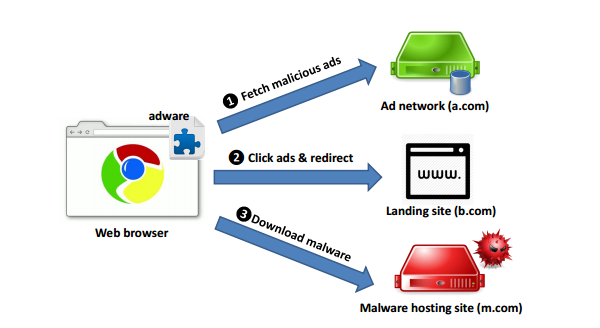
\includegraphics[height=10cm,width=25cm]{intro.png}
\caption{An Example of simple Malicious Extension}
\end{figure}

\end{block}

%------------------------------------------------



%----------------------------------------------------------------------------------------

\end{column} % End of the first column

\begin{column}{\sepwid}\end{column} % Empty spacer column

\begin{column}{\twocolwid} % Begin a column which is two columns wide (column 2)
\begin{block}{Dataset Collection}
\end{block}

%----------------------------------------------------------------------------------------
%	MATERIALS
%----------------------------------------------------------------------------------------

\vspace{-1in}
Dataset collection was a major challenge in this domain since there has not been any extensive research or analysis in this field so far. For this purpose, we developed a chrome extension scans for a link to an extension on the page and uploads it to a central repository. This extension was installed by some volunteers. Around 1600 extensions were collected over a total of 2 months. Also, 1300 benign extensions were collected from chrome's store.


%----------------------------------------------------------------------------------------


\vspace{0.1in}

 % End of the split of column 2 - any content after this will now take up 2 columns width
\begin{block}{Methodology}
\begin{figure}
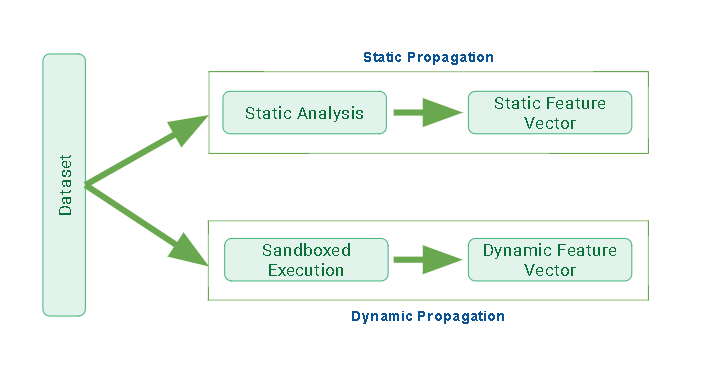
\includegraphics[height=29cm,width=50cm]{flow.png}
\caption{Flow Diagram}
\end{figure}
Analysis of an extension can be either static or dynamic.\\*
Static analysis comprises of features extracted without actually executing it, eg. Source url, permissions etc.\\*
For dynamic analysis, we need to run the extension in a sandboxed environment and log its behaviour, eg. data sent, page content modified, etc.\\*
We will extract a feature vector corresponding to an extension using both static and dynamic analysis.\\*
Next step is to determine an appropriate model and train it using the training set. We decided to use SVM because of its success in previous work on malware analysis.

\end{block}

%----------------------------------------------------------------------------------------
%	IMPORTANT RESULT
%----------------------------------------------------------------------------------------

% \begin{alertblock}{Important Result}

% Lorem ipsum dolor \textbf{sit amet}, consectetur adipiscing elit. Sed commodo molestie porta. Sed ultrices scelerisque sapien ac commodo. Donec ut volutpat elit.

% \end{alertblock} 

%----------------------------------------------------------------------------------------
\begin{block}{SVM Classification}
We will use various features in our model. For static analysis we will use features  like the size of the js/binary files and the permissions the application is asking   like opening tabs, some socket io permissions etc. For Dynamic analysis we will use features like the network logs captured, what all files the application is writing and reading in our system and the sequence of file execution etc.
\end{block}
\end{column} % End of the second column

\begin{column}{\sepwid}\end{column} % Empty spacer column

\begin{column}{\onecolwid} % The third column



%----------------------------------------------------------------------------------------
%	Image
%----------------------------------------------------------------------------------------
\begin{block}{}
% Please add the following required packages to your document preamble:
% \usepackage[table,xcdraw]{xcolor}
% If you use beamer only pass "xcolor=table" option, i.e. \documentclass[xcolor=table]{beamer}
\begin{figure}
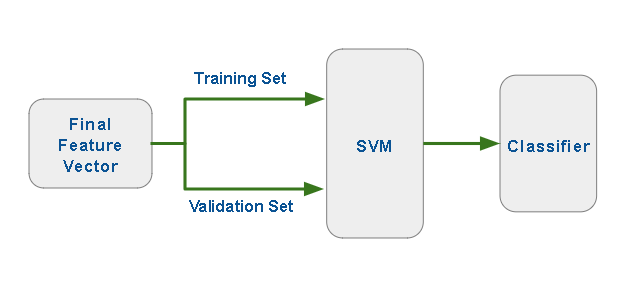
\includegraphics[scale=0.98]{ml.png}
\caption{SVM Classifier on Dataset}
\end{figure}
\end{block}

%----------------------------------------------------------------------------------------
%	CONCLUSION
%----------------------------------------------------------------------------------------
\vspace{-0.7in}
\begin{block}{Conclusion}

We explore the novel model for Supervised Learning of features of the browser extensions using Support Vector Machine(SVM) classification Model. We dig into behaviour of malicious extensions(both static and dynamic malwares) by creating a sandboxed environment and learn patterns and repetitions based on the activities and executions performed by the maline extensions onto the target system. Finally, we were able to build a classifier which can predict wheter an extension is harmful or not and thus successfully classify the threat level.

\end{block}

%----------------------------------------------------------------------------------------
%	ADDITIONAL INFORMATION
%----------------------------------------------------------------------------------------

% \begin{block}{Additional Information}

% Maecenas ultricies feugiat velit non mattis. Fusce tempus arcu id ligula varius dictum. 
% \begin{itemize}
% \item Curabitur pellentesque dignissim
% \item Eu facilisis est tempus quis
% \item Duis porta consequat lorem
% \end{itemize}

% \end{block}

%----------------------------------------------------------------------------------------
%	REFERENCES
%----------------------------------------------------------------------------------------

\begin{block}{References}
\nocite{*}
\small{\bibliographystyle{ieeetr}
\bibliography{sample}\vspace{0.75in}}
\end{block}

%----------------------------------------------------------------------------------------
%	ACKNOWLEDGEMENTS
%----------------------------------------------------------------------------------------

\setbeamercolor{block title}{fg=red,bg=white} % Change the block title color


%----------------------------------------------------------------------------------------
%	CONTACT INFORMATION
%----------------------------------------------------------------------------------------

\setbeamercolor{block alerted title}{fg=black,bg=norange} % Change the alert block title colors
\setbeamercolor{block alerted body}{fg=black,bg=white} % Change the alert block body colors



%----------------------------------------------------------------------------------------

\end{column} % End of the third column

\end{columns} % End of all the columns in the poster

\end{frame} % End of the enclosing frame

\end{document}
